\documentclass[a4paper, 12pt]{article}
\usepackage{graphicx}
\graphicspath{{images/}}
\usepackage{listings}
\usepackage[english]{babel}
\usepackage{caption}
\usepackage{color}
\usepackage{array}


\title{Homework 2}
\author{Nasir Mohammad Khalid}

\makeatletter
\let\thetitle\@title
\let\theauthor\@author
\let\thedate\@date
\makeatother

\definecolor{codegreen}{rgb}{0,0.6,0}
\definecolor{codegray}{rgb}{0.5,0.5,0.5}
\definecolor{codepurple}{rgb}{0.58,0,0.82}
\definecolor{backcolour}{rgb}{0.95,0.95,0.92}

\lstdefinestyle{mystyle}{
    backgroundcolor=\color{backcolour},   
    commentstyle=\color{codegreen},
    keywordstyle=\color{magenta},
    numberstyle=\tiny\color{codegray},
    stringstyle=\color{codepurple},
    basicstyle=\scriptsize,
    breakatwhitespace=false,         
    breaklines=true,                 
    captionpos=b,                    
    keepspaces=true,                 
    numbers=left,                    
    numbersep=1pt,                  
    showspaces=false,                
    showstringspaces=false,
    showtabs=false,                  
    tabsize=1
}

\lstset{style=mystyle}

\newenvironment{conditions}
  {\par\vspace{\abovedisplayskip}\noindent\begin{tabular}{>{$}l<{$} @{${}={}$} l}}
  {\end{tabular}\par\vspace{\belowdisplayskip}}

\begin{document} 
    \begin{titlepage}
        \centering
        \vspace*{0.5 cm}
        
\includegraphics[scale = 0.60]{logo.png}\\[1.0 cm]	% University Logo
        \textsc{\LARGE American University of Sharjah}\\[1.0 cm]
        \textsc{\Large ELE494-09}\\[0.2 cm]	
        \textsc{\Large Deep Networks in Machine Learning}\\[0.5 cm]			% Course Code
        \rule{\linewidth}{0.2 mm} \\[0.4 cm]
        { \huge \bfseries \thetitle}\\
        \rule{\linewidth}{0.2 mm} \\[1.5 cm]
        
        \textsc{\Large{\theauthor}}\\[0.3 cm]
        \textsc{\Large{65082}}\\[0.3 cm]
        \textsc{\Large{\thedate}}\\[1.5 cm]

        \textmd{Submitted To: \itshape{Dr.Usman Tariq}}
    \end{titlepage}

    \clearpage
    \tableofcontents
    \listoffigures
    \lstlistoflistings
    \clearpage

    \section{Task 1: Backpropagation}

    \subsection{Q1}

    The goal of this part to develop a theoretical understanding of how do you get the expressions with
    backpropagation algorithm. Suppose you have a three layer fully connected neural network (input layer,
    hidden layer and output layer). Following are some further "specifications":

    \begin{itemize}
        \item The input feature vectors are d dimensional (you can think of these as MNIST images, attened as vectors)
        \item There are N feature vectors in you training dataset
        \item There are H hidden nodes and K output nodes (for K mutually exclusive classes).
        \item This neural network is to be trained for classification under cross-entropy loss function
    \end{itemize}

    Derive the equations for batch gradient updates for the input-to-hidden unit weights and hidden-to-output
    unit weights. Is it wise to use a learning rate parameter? Why?

    \subsection{Background to Answer}
    
    Based on the specifications given we can assume the architecture of the neural network to be as follows:

    \begin{figure}[h!]
        \centering
        \captionsetup{justification=centering}
        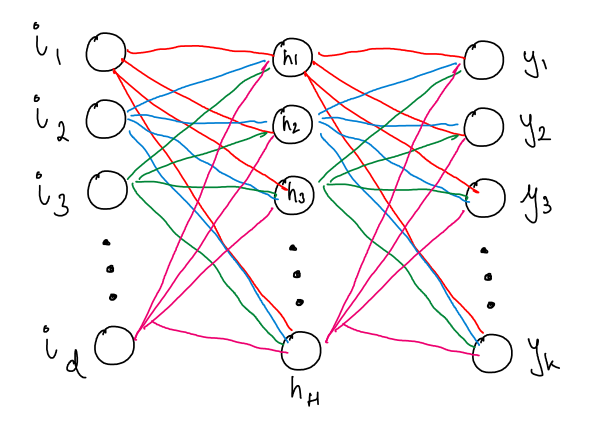
\includegraphics[scale = 0.37]{1.png}
        \caption{Representation of the neural network}
    \end{figure}
    
    The output of the node 'h' of hidden layer will be calculated using the sigmoid activation function and is given as follows:

    \begin{equation}
        Z_h = \sum_{n=1}^{d} i_n * w_{nh} + b_h
    \end{equation}

    \begin{equation}
        O_h = \frac{1}{1+e^{Z_h}}
    \end{equation}

    \begin{center}
        \begin{conditions}
            $$Z_h$$     &   Input to the sigmoid function of node 'h' \\
            $$O_h$$     &   Output of the sigmoid function of the node 'h' \\   
            $$b_h$$     &   Bias of the input to node h \\   
            $$w_{nh}$$  &   Weight between input node $$n$$ and the hidden node $$h$$\\
        \end{conditions}
    \end{center}
    
    The output of the node 'o' of the final layer will be calculated using the softmax function and it will be given as follows:
    
    \begin{equation}
        Z_o = \sum_{n=1}^{h} O_{n} * w_{no} + b_o
    \end{equation}

    \begin{equation}
        Y_o = \frac{e^{Z_o}} {\sum_{j=1}^{k} e^{Z_j}}
    \end{equation}

    \begin{center}
        \begin{conditions}
            $$Z_o$$     &   Input to the softmax function of node 'o' \\
            $$Y_o$$     &   Output of the 'o'th output layer \\
            $$b_o$$     &   Bias of the Output node 'o' \\
            $$w_{no}$$  &   Weight between the 'n'th hidden node to the 'o'th output node\\
        \end{conditions}
    \end{center}

    The output layer will give values between 0 and 1 only. The error function is the cross-entropy function. Since the output consists of K mutually exclusive classes then we can take the label for the feature vectors to be of a matrix of length K
    and it contains a 1 at the appropriate label. Then the cross entropy loss function is given as:

    \begin{equation}
        E = - \sum_{i=1}^{k} L_i * log(Y_i)
    \end{equation}
    \begin{center}
        \begin{conditions}
            $$E$$       &   Error value from the cross-entropy function \\
            $$L_k$$     &   Value of the label at the 'k'th index \\   
            $$Y_k$$     &   Output of output node 'k'\\
        \end{conditions}
    \end{center}

    Now we want to get the derivative of the error with respect to the first set of weights between the hidden layer and output layer:

    \begin{equation}
        \frac{\partial E}{\partial w_{hk}} = \frac{\partial E}{\partial Z_k} * \frac{\partial Z_k}{\partial w_{hk}}
    \end{equation}

    \begin{center}
        \begin{conditions}
            $$\frac{\partial E}{\partial w_{hk}}$$      &   $\partial$ of Error function w.r.t weights between hidden and output layer \\[0.3 cm]
            $$\frac{\partial E}{\partial Z_k}$$         &   $\partial$ of the Error function with respect to the input to the softmax\\[0.3 cm]
            $$\frac{\partial Z_k}{\partial w_{hk}}$$    &   $\partial$ of input to softmax w.r.t  weights between hidden and output layer\\[0.3 cm]
        \end{conditions}
    \end{center}

    The derivative of the softmax function $Y_o$ with respect to the input of the softmax function $Z_k$ is obtained through the quotient rule and is given by:
    
    \begin{equation}
        \frac{\partial Y_o}{\partial Z_k} = Y_k * (1-Y_j) = Y_k * (1-Y_k) \quad {when \quad j = k}
    \end{equation}

    \begin{equation}
        \frac{\partial Y_o}{\partial Z_k} = - Y_j * Y_k \quad {when \quad j \neq k}
    \end{equation}\\

    The derivative of the error with respect to the input to the softmax can will consist of two parts. The first is when $i = k$ (in summation) and the second is when they are not the same:

    \begin{equation}
        \frac{\partial E}{\partial Z_k} = - \sum_{i=1}^{k} L_i * \frac{\partial log(Y_i)}{\partial Y_i} * \frac{\partial Y_i}{\partial Z_k} 
    \end{equation}

    \begin{equation}
        \frac{\partial E}{\partial Z_k} = -L_k * \frac{\partial log(Y_k)}{\partial Y_k} * \frac{\partial Y_k}{\partial Z_k} = -L_k * (1-Y_j) \quad {when \quad i = k}
    \end{equation}

    \begin{equation}
        \frac{\partial E}{\partial Z_k} = - \sum_{i \neq k} L_i * \frac{\partial log(Y_i)}{\partial Y_i} * \frac{\partial Y_i}{\partial Z_k} =  \sum_{i \neq k} L_i * Y_j \quad {when \quad i \neq k}
    \end{equation}

    We take the summation of both cases to get the final derivative of error with respect to the input to the softmax function:

    \begin{equation}
        \frac{\partial E}{\partial Z_k} = -L_k * (1-Y_j) + \sum_{i \neq k} L_i * Y_j
    \end{equation}
    
    \begin{equation}
        \frac{\partial E}{\partial Z_k} = Y_j * (L_k + \sum_{i \neq k} L_i) - L_k
    \end{equation}
    
    but $(L_k + \sum_{i \neq k} L_i)$ is equal to 1 as it is all the intended outputs added up. Due to the fact that the outputs are always probabilities their sum will give 1 and therefore we get the final expression:

    \begin{equation}
        \frac{\partial E}{\partial Z_k} = Y_j - L_k = Y_k - L_k
    \end{equation} 

    \begin{center}
        \begin{conditions}
            $$\frac{\partial E}{\partial Z_k}$$      &   $\partial$ of Error function w.r.t input to the softmax function \\[0.3 cm]
            $$Y_k$$                                  &   It is the final output of the output neuron\\[0.3 cm]
            $$L_k$$                                  &   It is the intended output of the output neuron \\[0.3 cm]
        \end{conditions}
    \end{center}

    Similarly we the derivative of the input to the softmax with respect to the weights. Here $O_h$ is the output of the hidden layer:

    \begin{equation}
        \frac{\partial Z_k}{\partial w_{hk}} = O_h
    \end{equation}

    \subsection{A1: Gradient Update for hidden-to-output weights}

    The final answer is given by: 

    \begin{equation}
        \frac{\partial E}{\partial w_{hk}} = \frac{\partial E}{\partial Z_k} * \frac{\partial Z_k}{\partial w_{hk}} = (Y_k - L_k) * O_h
    \end{equation}
    
    \begin{center}
        \begin{conditions}
            $$\frac{\partial E}{\partial w_{hk}}$$   &   $\partial$ of Error function w.r.t weights between hidden-output \\[0.3 cm]
            $$Y_k$$                                  &   It is the final output of the output neuron\\[0.3 cm]
            $$L_k$$                                  &   It is the intended output of the output neuron \\[0.3 cm]
            $$O_h$$                                  &   It is the final output of the hidden neuron\\[0.3 cm]
        \end{conditions}
    \end{center}
    
    \subsection{A1: Gradient Update for input-to-hidden weights}

    Here we further extend the partial derivatives until we get the change in error with respect to the input-hidden weights
    \begin{equation}
        \frac{\partial E}{\partial w_{ih}} = \frac{\partial E}{\partial Z_k} * \frac{\partial Z_k}{\partial O_h} * \frac{\partial O_h}{\partial Z_h} * \frac{\partial Z_h}{\partial w_{ih}}
    \end{equation}

    \begin{center}
        \begin{conditions}
            $$\frac{\partial E}{\partial w_{ih}}$$   &   $\partial$ of Error function w.r.t weights between input-hidden \\[0.3 cm]
            $$\frac{\partial E}{\partial Z_k}$$      &   $\partial$ of Error function w.r.t input to softmax \\[0.3 cm]
            $$\frac{\partial Z_k}{\partial O_h}$$    &   $\partial$ of Input to softmax w.r.t output of hidden \\[0.3 cm]
            $$\frac{\partial O_h}{\partial Z_h}$$    &   $\partial$ of Output of hidden w.r.t input to sigmoid\\[0.3 cm]
            $$\frac{\partial Z_h}{\partial w_{ih}}$$ &   $\partial$ of Input to sigmoid w.r.t weight between input and hidden \\[0.3 cm]
        \end{conditions}
    \end{center}

    We already obtained the first term $ \frac{\partial E}{\partial Z_k} $ in section 1.4 and the rest are derived below. The first one (18) where $w_hk$ is the weight between hidden and output layer

    \begin{equation}
        \frac{\partial Z_k}{\partial O_h} = w_{hk}
    \end{equation}

    (19) is derivative of the sigmoid function

    \begin{equation}
        \frac{\partial O_h}{\partial Z_h} = O_h * (1- O_h)
    \end{equation}

    Here $ i_n $ is the input to the network

    \begin{equation}
        \frac{\partial Z_h}{\partial Z_h} = i_n
    \end{equation}

    Combining all of these together gives the final equation for the change in error with respect to the weights between input-hidden layer.

    \begin{equation}
        \frac{\partial E}{\partial w_{ih}} = (Y_k - L_k) * w_{hk} * Oh * (1-O_h) * i_n
    \end{equation}

    \begin{center}
        \begin{conditions}
            $$\frac{\partial E}{\partial w_{ih}}$$   &   $\partial$ of Error function w.r.t weights between input-hidden \\[0.3 cm]
            $$Y_k$$                                  &   Output of the final neuron\\[0.3 cm]
            $$L_k$$                                  &   Intended output of final neuron\\[0.3 cm]
            $$w_{hk}$$                               &   Weights between hidden and output layer\\[0.3 cm]
            $$O_h$$                                  &   Output of hidden neuron\\[0.3 cm]
            $$i_n$$                                  &   Input of first neuron\\[0.3 cm]
        \end{conditions}
    \end{center}

\end{document} 